\chapter{Special Functions and Properties}
This appendix covers the basics of some of the special functions that arise when discussing the properties of some operators in quantum mechanics and formulae used.
\section{Legendre Polynomials and Spherical Bessel Functions}\label{app:Bessel}
\begin{equation}
	Y_{\ell}^m(\theta,\phi) = \frac{(-1)^{{\ell}l+m}}{(2\ell)!!}\bigg[ \frac{(2\ell+1)(\ell-m)}{4\pi(\ell+m)!}\bigg](\sin\theta)^m\frac{\text{d}^{\ell+m}}{(d\cos\theta)^{\ell+m}}[(\sin\theta)^{2\ell}]\exp{i m\phi},
\end{equation}
which satisfy
\begin{equation}
	Y_\ell^{*m}=(-1)^m Y_{l}^{-m}.
\end{equation}
The spherical harmonics are connected to the Legendre polynomials
\begin{equation}
	P_\ell(\cos\theta) = \bigg[ \frac{4\pi}{2\ell+1} \bigg]^{1/2}Y_{l}^0(\theta).
\end{equation}
Another important feature of spherical harmonics is that they form a complete set of functions over the unit sphere. Furthermore, they form an orthonormal set
\begin{equation}\label{orthset}
	\int \text{d}\Omega \, Y_\ell^{*m} Y_{l'}^{m'} = \delta_{mm'}\delta_{ll'}.
\end{equation}
Also, there exists an addition theorem for spherical harmonics
\begin{equation}\label{addition}
	\sum_{m=-\ell} Y_\ell^{*m}(\theta,\phi)Y_\ell^{m}(\theta'.\phi') = \bigg( \frac{2\ell+1}{4\pi}\bigg)^{1/2}Y_\ell^0(\alpha).
\end{equation}
The wave function of a plane wave with wave number $k$ propagating along the $z$ axis can be described by
\begin{align} \label{planewave}
	\text{e}^{ikz}  &= \text{e}^{ikr \cos(\theta)}  \\
	&= \sum_{\ell=0}^\infty A_\ell(r)Y_{\ell,0}(\theta),
\end{align}
where
\begin{equation} \label{besselcoef}
	A_\ell(r) = \int \text{d}\Omega \, Y_{\ell,0}^*(\theta)\text{e}^{ikr\cos(\theta)}  = i^\ell\sqrt{4\pi(2\ell+1)}j_\ell(kr),
\end{equation}
where the last equality shows the coefficient $A_\ell(r)$ can be expressed in terms of a spherical Bessel function $j_\ell(kr)$. Using the addition theorem equation \eqref{planewave} yields the decomposition of a plane wave into spherical Bessel functions
\begin{equation} \label{sphericalbesseldecomp}
	\text{e}^{i\vec{k}\cdot\vec{r}} = 4\pi \sum_{\ell,m}i^\ell j_\ell(kr)Y_\ell^{m*}(\theta,\phi)Y_\ell^{m}(\theta,\phi)
\end{equation}
\section{Bessel Functions}\label{app:Besselfunctions}
Considering the free radial Schrödinger equation
\begin{equation} \label{freesch}
		\bigg( \frac{\text{d}^2}{\text{d}r^2}-\frac{\ell(\ell+1)}{r^2}+p^2\bigg)y(r) = 0, \quad p=\sqrt{2mE},
\end{equation}
which is an ordinary, linear, second-order differential equation and has two linearly independent solutions \cite{TaylorScattering}. The solutions that are relevant in a physics context must vanish at vanish at the origin. If we consider the limit where $r\rightarrow0$ the centrifugal term $\ell(\ell+1)$ will dominate the energy term $p^2$ and hence the solutions will be similar to letting $p=0$ for which the solutions are $r^{\ell+1}$ and $r^{-\ell}$. From these two considerations we know the physically acceptable solution to equation \eqref{freesch} must be on the form $r^{\ell+1}$. These are the functions
\begin{align} \label{Riccati}
		\hat{j}_\ell(pr) &\equiv prj_\ell(pr) \equiv \bigg(\frac{\pi pr}{2} \bigg)^{1/2} J_{\ell+1/2}(pr) \\
		&=(pr)^{\ell+1}\sum_{n=0}^\infty \frac{(-pr/2)^n}{n!(2\ell+2n+1)!!},
\end{align}
where the spherical Bessel functions are denoted $j_\ell(pr)$ and the ordinary Bessel functions are denoted $J_\lambda(pr)$. It is possible to express any function $f(r)$ as the weighted sum of Bessel functions. This is known as the Hankel transform given by
\begin{equation} \label{HankelTransform}
	F_\lambda(k) = \int_0^\infty \text{d}r \, f(r) J_\lambda(kr)r,
\end{equation}
with the inverse Hankel function defined as 
\begin{equation} \label{invHankel}
	f(r) = \int_0^\infty \text{d}k \, F_\lambda(k)J_\lambda(kr)k.
\end{equation}
Both equation \eqref{HankelTransform} and equation \eqref{invHankel} can be expressed in terms of the spherical Bessel functions from equation \eqref{Riccati} and this is essentially what is done in equation \eqref{unitbob} which means the wave function $\phi(r)$ is defined through the Hankel transforms.
\section{Coulomb Wave Functions}\label{sec:Coulomb}
The Coulomb wave equation for a charged particle with arbitrary angular momentum and charge is given by 
\begin{equation} \label{Coulomb1}
	\nabla^2\psi +\left( k^2-\frac{2\mu}{\hbar^2}V(r)\right)\psi = 0,
\end{equation}
where $\mu$ is the reduced mass of the system. The radial wave function $u(r)$ satisfied the following differential equation
\begin{equation} \label{Coulomb2}
	\frac{\text{d}^2 u_\ell}{\text{d}r^2}+\left( k^2-\frac{\ell(\ell+1)}{r^2}-\frac{2\mu}{\hbar^2}\frac{Ze^2}{r}\right)u_\ell=0,
\end{equation}
where $Z$ is the product of the charges. Two independent solutions can be found to equation \eqref{Coulomb2} -- these are called the regular and irregular Coulomb wave functions denoted $F_\ell(r)$ and $G_\ell(r)$ respectively. The regular Coulomb wave function $F_\ell(r)$ is a real function that vanishes at $r=0$ and the behaviour of the function is described using a parameter $\eta$ which describes how strongly the Coulomb interaction is
\begin{equation} \label{etafactor}
	\eta = \frac{Zmc\alpha }{\hbar k},
\end{equation}
where $m$ is the mass of the particle, $k$ is the wave number and $\alpha$ is the fine structure constant. The solution to is given by
\begin{equation} \label{solCoul}
	F_\ell(\eta,kr) = C_\ell (\eta) (kr)^{\ell+1}\text{e}^{-ikr}  {}_1 F_1(\ell+1-i\eta,2\ell+2,2ikr),
\end{equation}
where ${}_1F_1(kr)$ is a confluent hypergeometric function and $C_\ell(\eta)$ is a normalization constant given by 
\begin{equation} \label{normalization}
	C_\ell(\eta) = \frac{2^\ell \text{e}^{-\pi\eta/2}\abs{\Gamma(\ell+1+i\eta)}}{(2\ell+1)!},
\end{equation}
where $\Gamma$ is the gamma function. For numerical purposes, it is useful to use the integral representation of equation \eqref{solCoul} \cite[eq. 33.7.1]{NIST} 
\begin{equation} \label{integralrep}
	F_\ell(\eta,\rho) = \frac{\rho^{\ell+1}2^\ell e^{i\rho-(\pi\eta/2)}}{|\Gamma(\ell+1+i\eta)|} \int_0^1 e^{-2i\rho t}t^{\ell+i\eta}(1-t)^{\ell-i\eta} \, \text{d}t.
\end{equation}
Some examples of equation \eqref{integralrep} are shown in figure \ref{fig:Coulombwavefunctions}.
\begin{figure}[H]
	\begin{sidecaption}{Coulomb wave functions. Both in the attractive and repulsive case. }[fig:Coulombwavefunctions]
		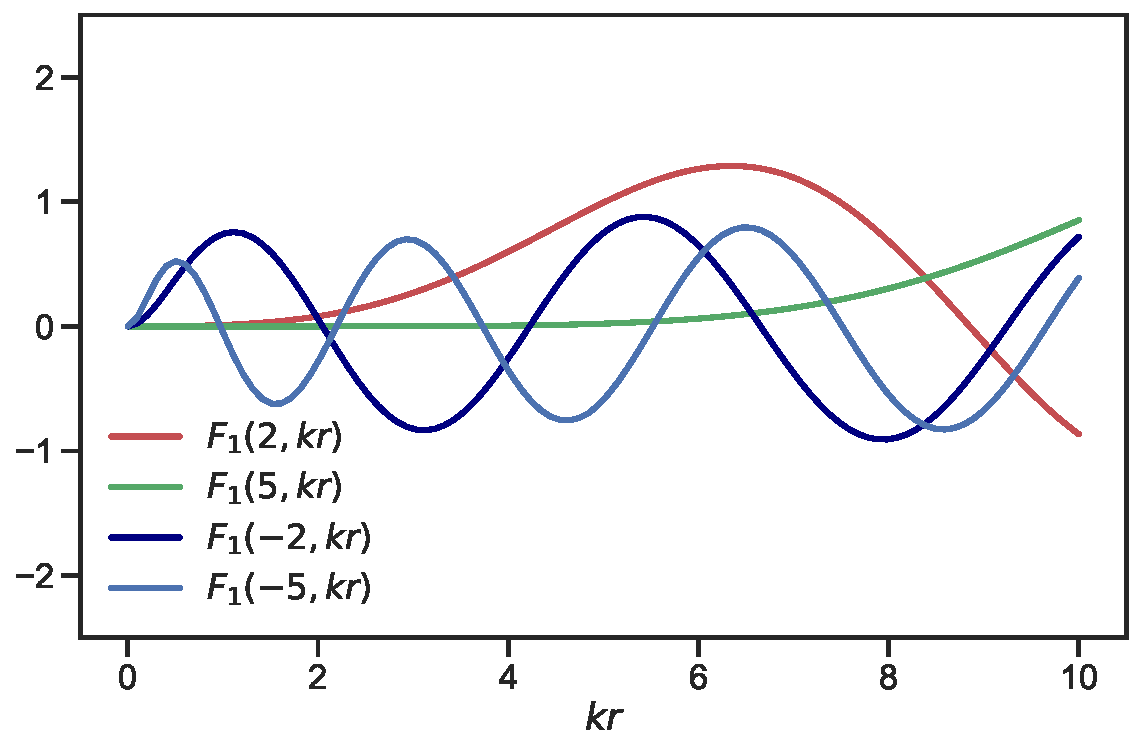
\includegraphics[width=\linewidth]{Figures/AttRepulCoulomb.pdf}
	\end{sidecaption}
\end{figure}
For particles without charge, we can ignore the Coulomb interaction in equation \eqref{Coulomb2} and the solution becomes \cite{Blatt}
\begin{equation} \label{solcharge}
	F_\ell(kr) = \left( \frac{\pi kr}{2} \right)^{1/2} J_{\ell+1/2}(kr)=kr j_\ell(kr), \quad \text{particles without charge}
\end{equation}
where $J_{\ell+1/2}$ is a Bessel function and $j_\ell$ is a spherical Bessel function. The limit as $\eta\rightarrow 0$ is shown on figure \ref{fig:Coulomblimit}
\begin{figure}[H]
	\begin{sidecaption}{Coulomb wave functions as $\eta\rightarrow 0$ which means the particles become neutral. In this case the Coulomb wave function becomes a spherical Bessel function. }[fig:Coulomblimit]
		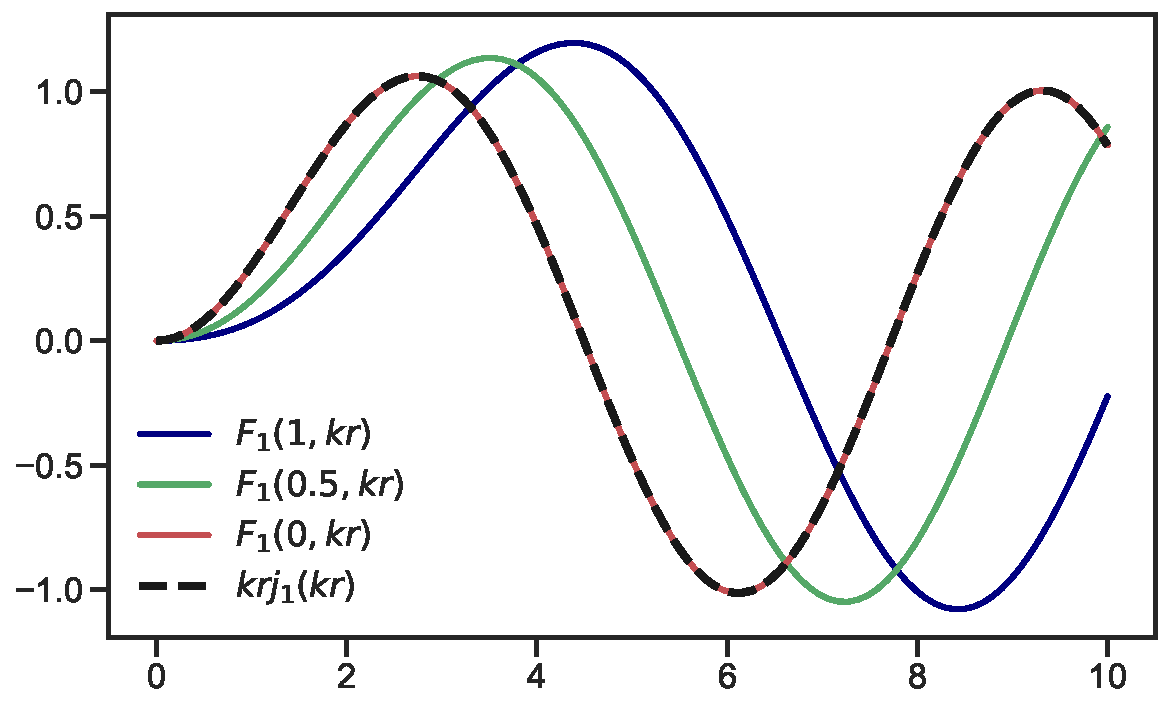
\includegraphics[width=\linewidth]{Figures/LimitBessel.pdf}
	\end{sidecaption}
\end{figure}

\chapter{Angular Distribution}\label{sec:Angular}
\begin{figure}[H]
	\begin{sidecaption}{Angular distribution with the parameters $S=86.2$ MeV and $b=3.8$ fm using the relativistic density of states }[fig:Angular0]
		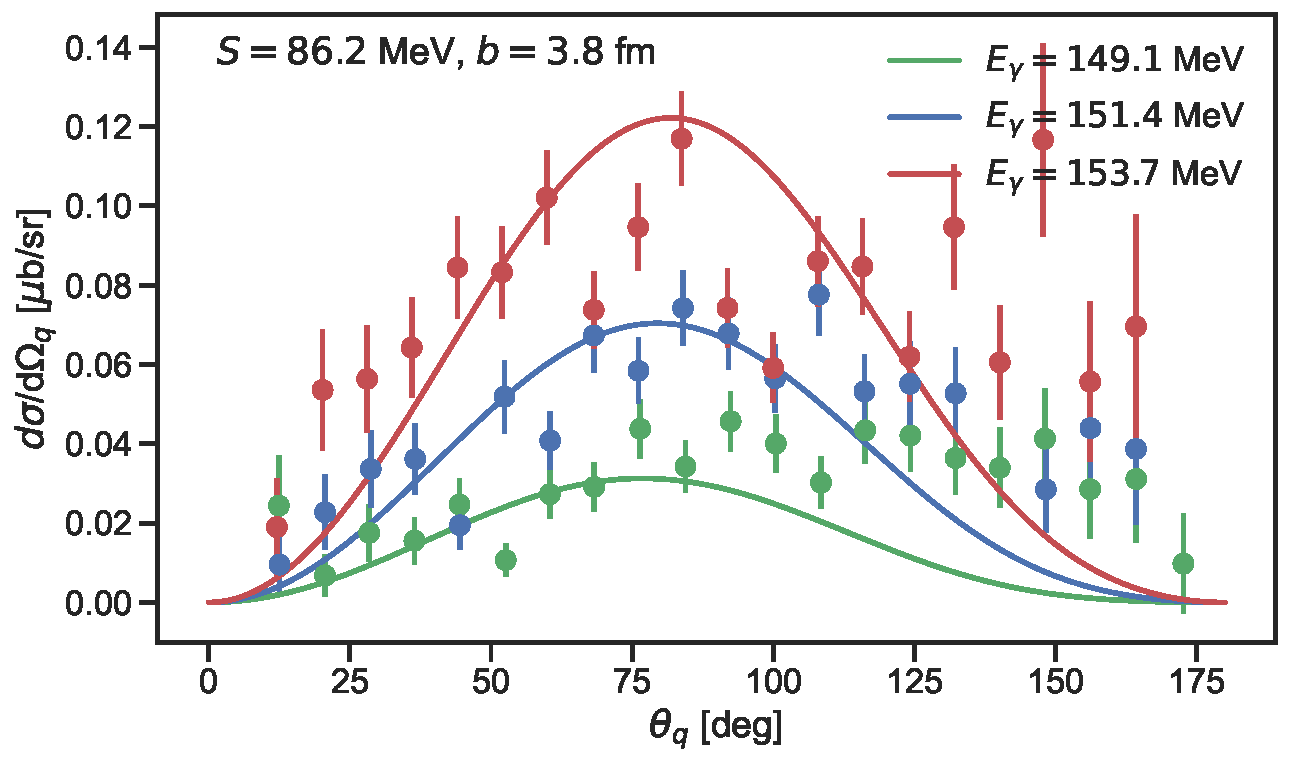
\includegraphics[width=\linewidth]{Figures/MultiDiffcross_rel.pdf}
	\end{sidecaption}
\end{figure}
\begin{figure}[H]
	\begin{sidecaption}{Angular distribution with the parameters $S=45.4$ MeV and $b=3.9$ fm using the relativistic density of state}[fig:Angular1]
		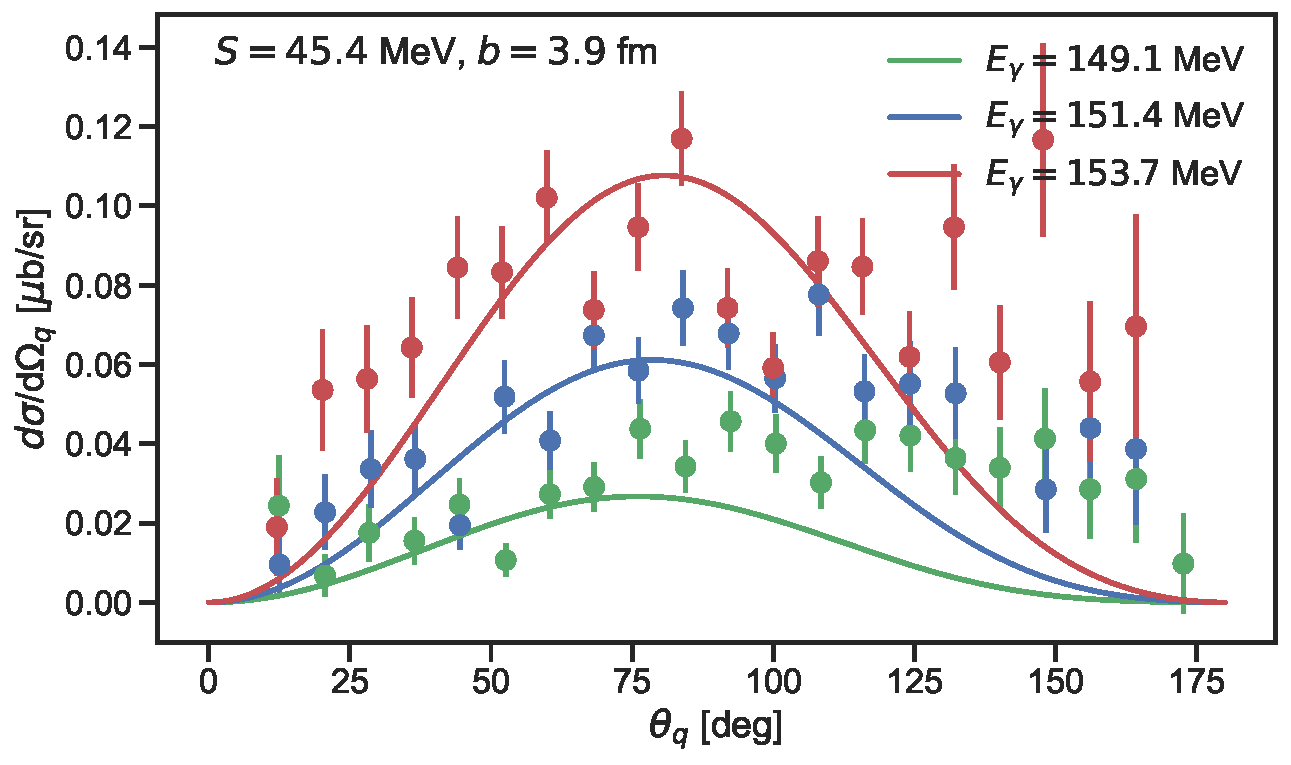
\includegraphics[width=\linewidth]{Figures/MultiDiffcross_rel_2.pdf}
	\end{sidecaption}
\end{figure}
\begin{figure}[H]
	\begin{sidecaption}{Angular distribution with the parameters $S=35$ MeV and $b=4.0$ fm using the relativistic density of state}[fig:Angular3]
		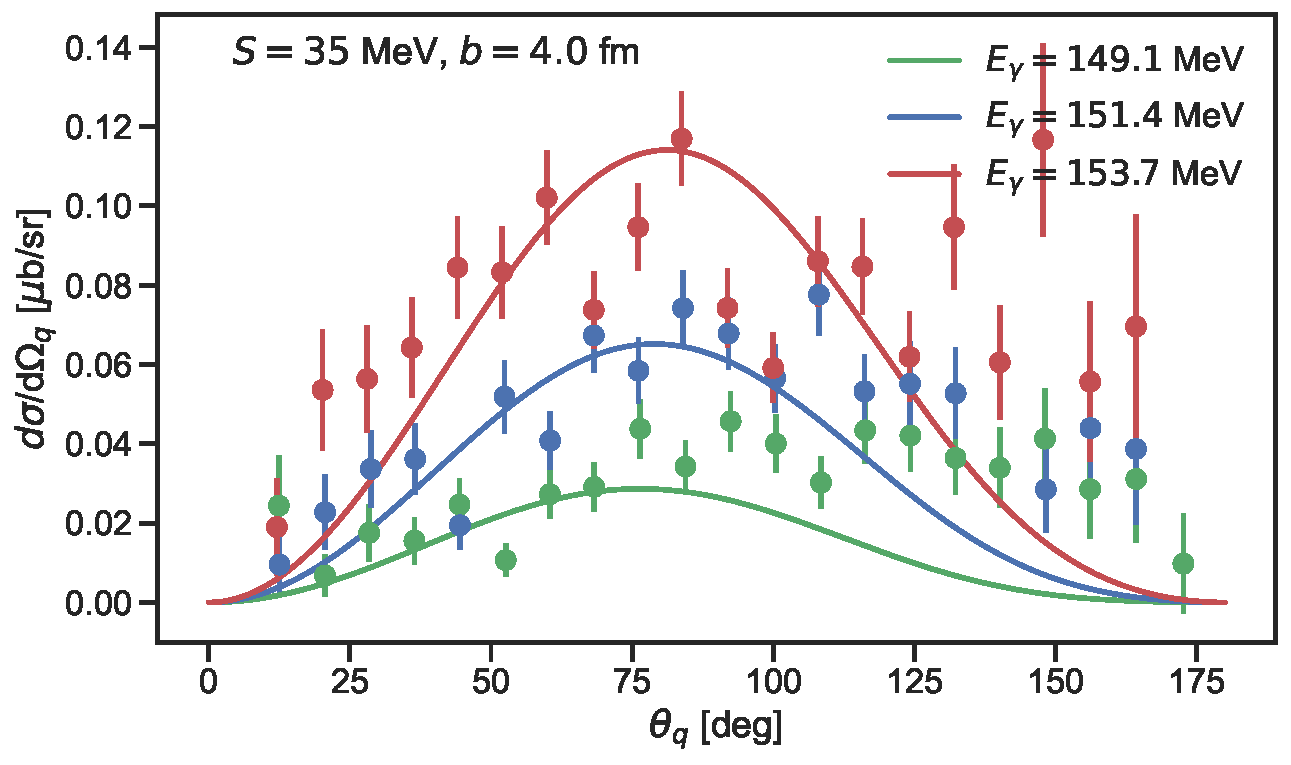
\includegraphics[width=\linewidth]{Figures/MultiDiffcross_rel_3.pdf}
	\end{sidecaption}
\end{figure}


\begin{figure}[H]
	\begin{sidecaption}{Angular distribution with the parameters $S=86.2$ MeV and $b=3.8$ fm using the non-relativistic density of states }[fig:Angular2]
		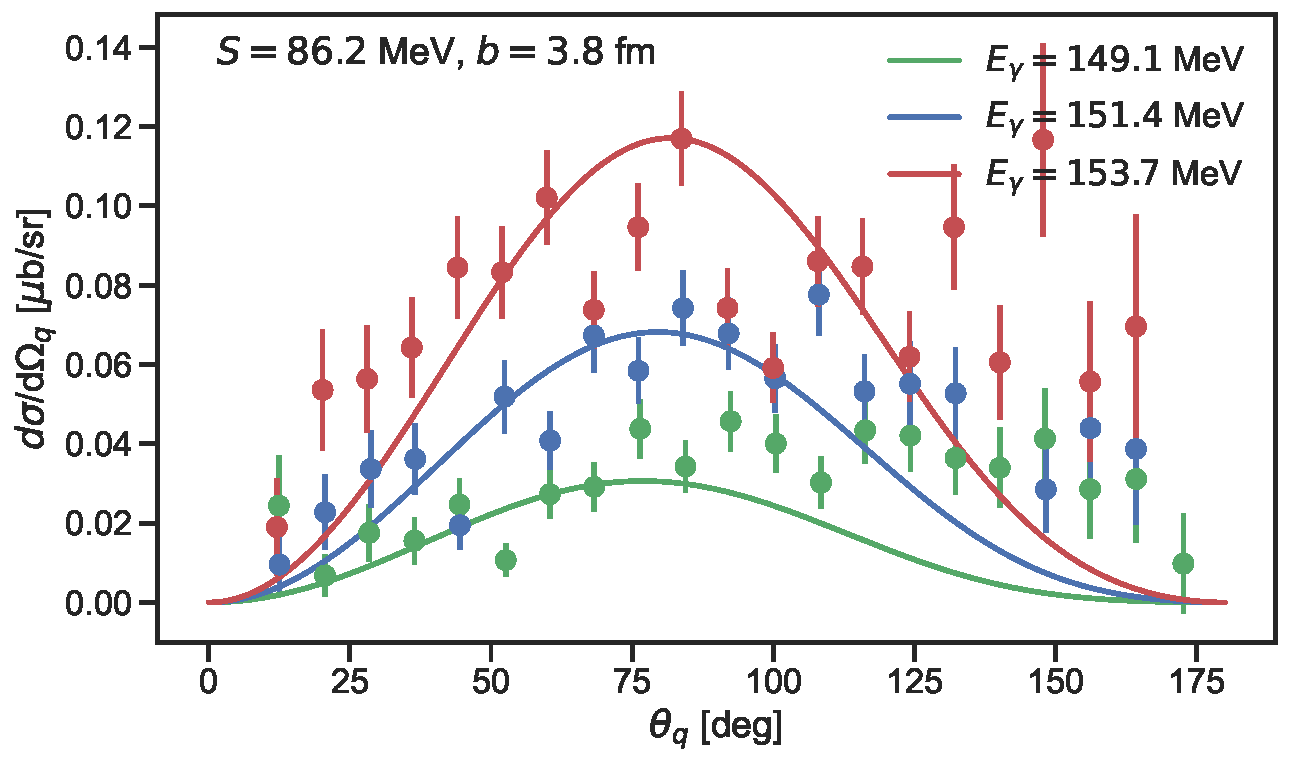
\includegraphics[width=\linewidth]{Figures/MultiDiffcross_nonrel_1.pdf}
	\end{sidecaption}
\end{figure}
\begin{figure}[H]
	\begin{sidecaption}{Angular distribution with the parameters $S=45.4$ MeV and $b=3.9$ fm using the non-relativistic density of state}[fig:Angular3]
		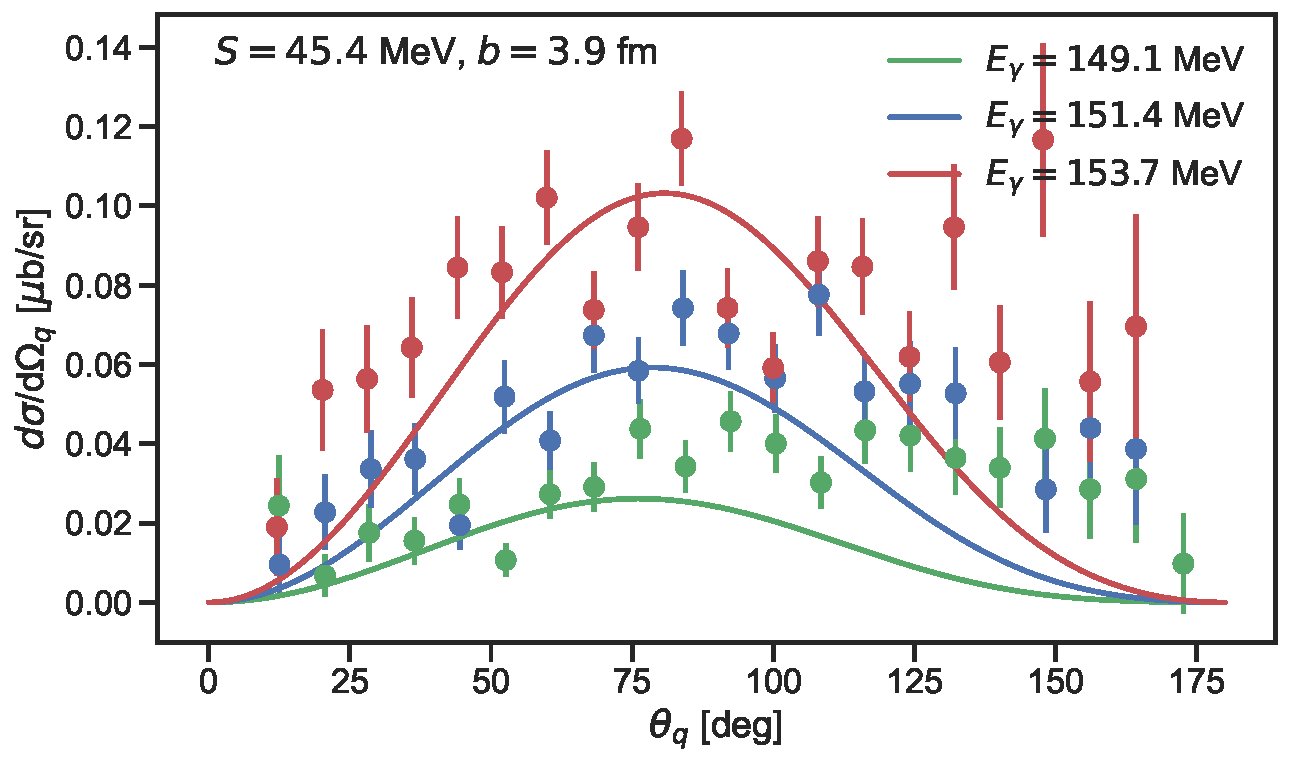
\includegraphics[width=\linewidth]{Figures/MultiDiffcross_nonrel_2.pdf}
	\end{sidecaption}
\end{figure}
\begin{figure}[H]
	\begin{sidecaption}{Angular distribution with the parameters $S=35$ MeV and $b=4.0$ fm using the non-relativistic density of state}[fig:Angular4]
		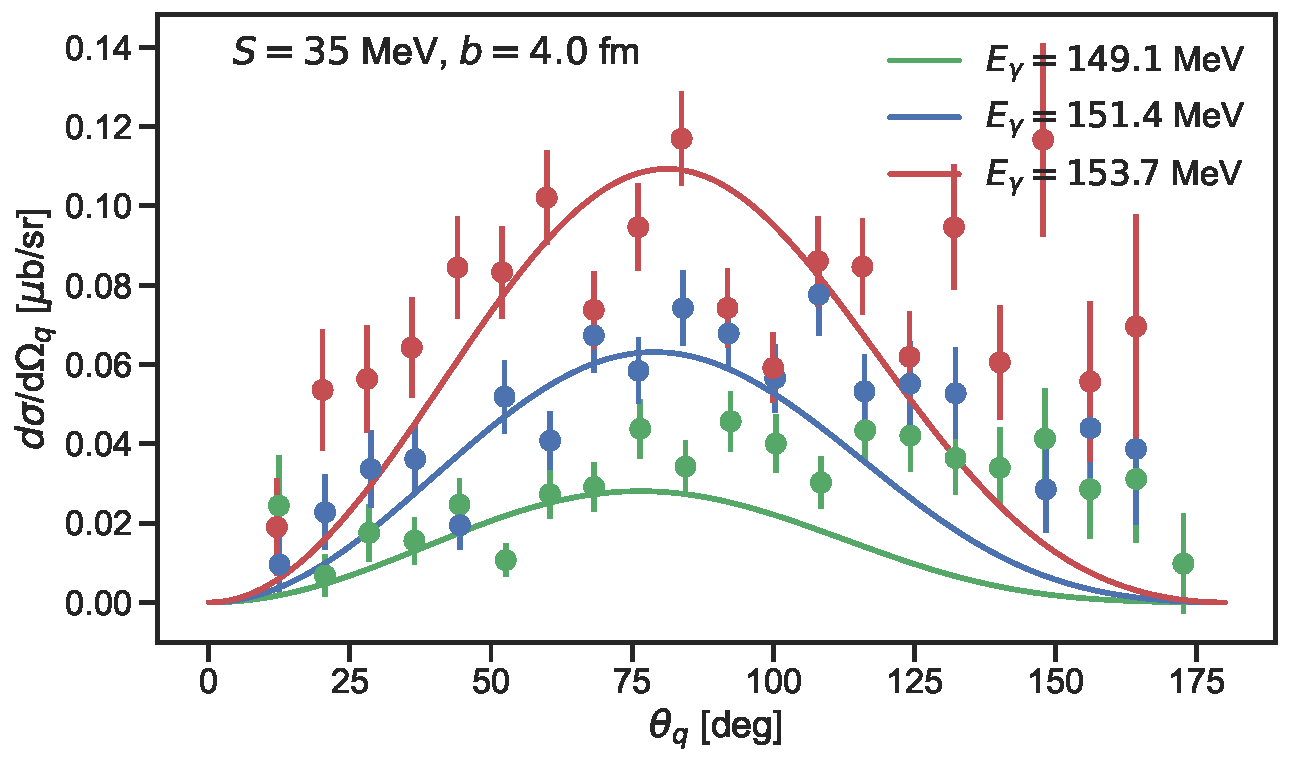
\includegraphics[width=\linewidth]{Figures/MultiDiffcross_nonrel_3.pdf}
	\end{sidecaption}
\end{figure}

